\documentclass[9pt,a4paper,twocolumn]{article}
\usepackage{fullpage, graphicx, url, enumitem, parskip, eurosym}

\newlist{tip}{itemize}{1}
\setlist[tip,1]{
  leftmargin=\dimexpr1.2cm+\labelsep\relax,
  label={\smash{\raisebox{-0.6\height}{
\includegraphics[width=1.5cm]{images/icons/tip.png}}}}
}

\newlist{arrow_red}{itemize}{1}
\setlist[arrow_red,1]{
  leftmargin=\dimexpr0.5cm+\labelsep\relax,
  label={\smash{\raisebox{-0.3\height}{
\includegraphics[width=0.5cm]{images/icons/arrow_red.png}}}}
}

\newlist{arrow_yellow}{itemize}{1}
\setlist[arrow_yellow,1]{
  leftmargin=\dimexpr0.5cm+\labelsep\relax,
  label={\smash{\raisebox{-0.3\height}{
\includegraphics[width=0.5cm]{images/icons/arrow_yellow.png}}}}
}

\newlist{arrow_blue}{itemize}{1}
\setlist[arrow_blue,1]{
  leftmargin=\dimexpr0.5cm+\labelsep\relax,
  label={\smash{\raisebox{-0.3\height}{
\includegraphics[width=0.5cm]{images/icons/arrow_blue.png}}}}
}

\newlist{arrow_green}{itemize}{1}
\setlist[arrow_green,1]{
  leftmargin=\dimexpr0.5cm+\labelsep\relax,
  label={\smash{\raisebox{-0.3\height}{
\includegraphics[width=0.5cm]{images/icons/arrow_green.png}}}}
}

\newlist{arrow_pink}{itemize}{1}
\setlist[arrow_pink,1]{
  leftmargin=\dimexpr0.5cm+\labelsep\relax,
  label={\smash{\raisebox{-0.3\height}{
\includegraphics[width=0.5cm]{images/icons/arrow_pink.png}}}}
}

\setlength{\parindent}{0em}
\setlength{\parskip}{1em}

\begin{document}


\includegraphics[width=\linewidth]{images/logo.png}

SkySight (https://skysight.io/) is an interactive soaring forecast tool developed by a team of meteorologists and Gliding World Champions. It combines the latest forecast modelling technologies with an intuitive user interface, to provide extremely high resolution forecasts and powerful flight planning tools. It has coverage for the majority of the world, and operates as a subscription service at 79\euro /yr at time of writing.
\subsection*{Local Soaring}
Using SkySight, it is very easy to check whether there will be good soaring weather. Thermals, wave, convergence and ridge lift are simply visualised with easy-to-read colour map overlays.

The simplest way to determine the forecast is to use the \textbf{Point Forecast} tool. This shows thermal conditions, cloud cover and significant weather in a convenient summary.

In complex or changable weather it may be best to check a few different points around the airfield, because local effects may be significant and affect the location you choose but not those immediately around.

\subsection*{Task Planning}
Task planning can often be complicated, with changing thermal conditions, cloud cover, overdevelopment, winds, airspace, convergences, wave and many other factors.

SkySight aims to make it as easy as possible to choose an effective task. To get started:

\begin{enumerate}
\item Look at the \textbf{Height of Thermals} and \textbf{Thermal Strength} throughout the day to determine the start and end of thermals, and get an overall picture of the task area.
\item Estimate a launch time and calculate the task window. Use the \textbf{Potential Flight Distance} as a guide for the maximum possible task length in the day.
\item Check the \textbf{Cu Cloudbase}, to see the areas there are expected to be Cumulus clouds. Areas with grey indicate possible small cloud formations, or some degree of uncertainty.
\item Check the \textbf{Cu Depth}. This shows the difference between the top of the thermals, and the condensation layer. Positive values indicate cumulus, whereas negative values indicate blue thermals. Values near zero may be sparse or small cumulus.
\item Use the \textbf{Boundary Layer Wind (Avg)} to find the average wind speed and direction. Wherever possible, consider lining up task legs with the prevailing wind.
\item Check the \textbf{Convergence} parameter to see if there are any lines of convergence or energy in your task area that you may be able to utilize in your task. Long lines of orange to red colour are ideal.
\item Check the \textbf{Cloud Cover}, \textbf{Overdevelopment} and \textbf{CAPE/Storms} for complex weather which may impact your task.
\item Review the \textbf{Satellite View} to confirm the current weather progression is matching the forecast, and consider accordingly. You can cross reference this easily with the \textbf{Forecast Satellite View} parameter.
\item Consider all of the information checked in the above steps. By following the best weather, input a task using the \textbf{Route Forecast} tool.
\item Validate understanding of the forecast by using the various \textbf{Point Tools} around the task area, to ensure full understanding of the weather development throughout the day.
\item If you are a power user, you may wish to review the \textbf{Point SkewT} and \textbf{Windgram Tool} around the task area for an indepth analysis.
\item Fly the task! Use the \textbf{IGC Upload} tool at the end of the day to analyse your flight.

\end{enumerate}
\subsection*{SkySight Interactive Tools}
SkySight includes many interactive tools. To use these tools:
\begin{enumerate}
\item Click on the desired power tool from the side menu.
\item Select a point on the map to see the forecast at that location.
\item For the Route and Wave forecasts, click again to define the task or cross-section.
\item If applicable, change the times using the top slider.
\item Close the forecast by clicking on the 
\includegraphics[height=12pt]{images/icons/exit.png}.
\end{enumerate}
\subsubsection*{
\includegraphics[height=15pt]{images/icons/skew-t.png} Point Skew-T}
The Skew-T log-P diagram is used to forecast the convective layer, upper atmospheric conditions, storm potentials and wind. SkySight generates an easy to read diagram for all points on the map.

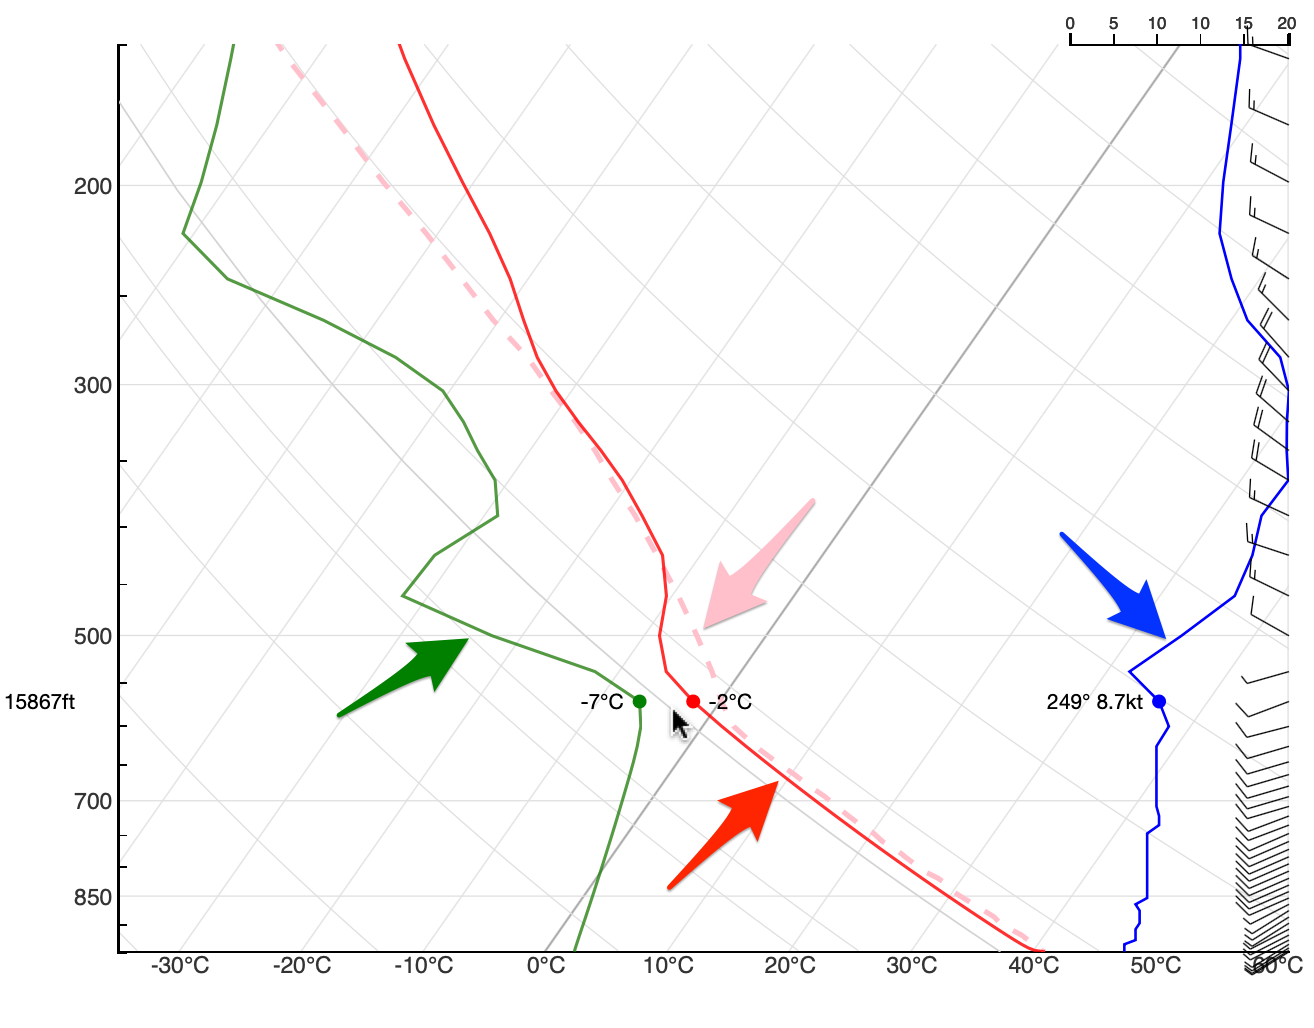
\includegraphics[width=\linewidth]{images/skew-t.png}

\begin{arrow_red}
\item \textbf{Temperature Curve} The forecast actual temperature changing with height.
\end{arrow_red}
\begin{arrow_green}
\item \textbf{Dewpoint Curve} The forecast dewpoint temperature changing with height.
\end{arrow_green}
\begin{arrow_blue}
\item \textbf{Wind Strength} The forecast wind strength changing with height. Wind barbs are also shown.
\end{arrow_blue}
\begin{arrow_pink}
\item \textbf{Virtual Parcel} A simulated hot air parcel rising through the boundary layer. Used to predict storm development potential and power.
\end{arrow_pink}

\subsubsection*{
\includegraphics[height=15pt]{images/icons/point_forecast.png} Point Forecast}

The point forecast tool allows the development of the conditions over the day to be summarised quickly. Cloud cover, thermal activity and temperatures are both visualised and displayed as values.

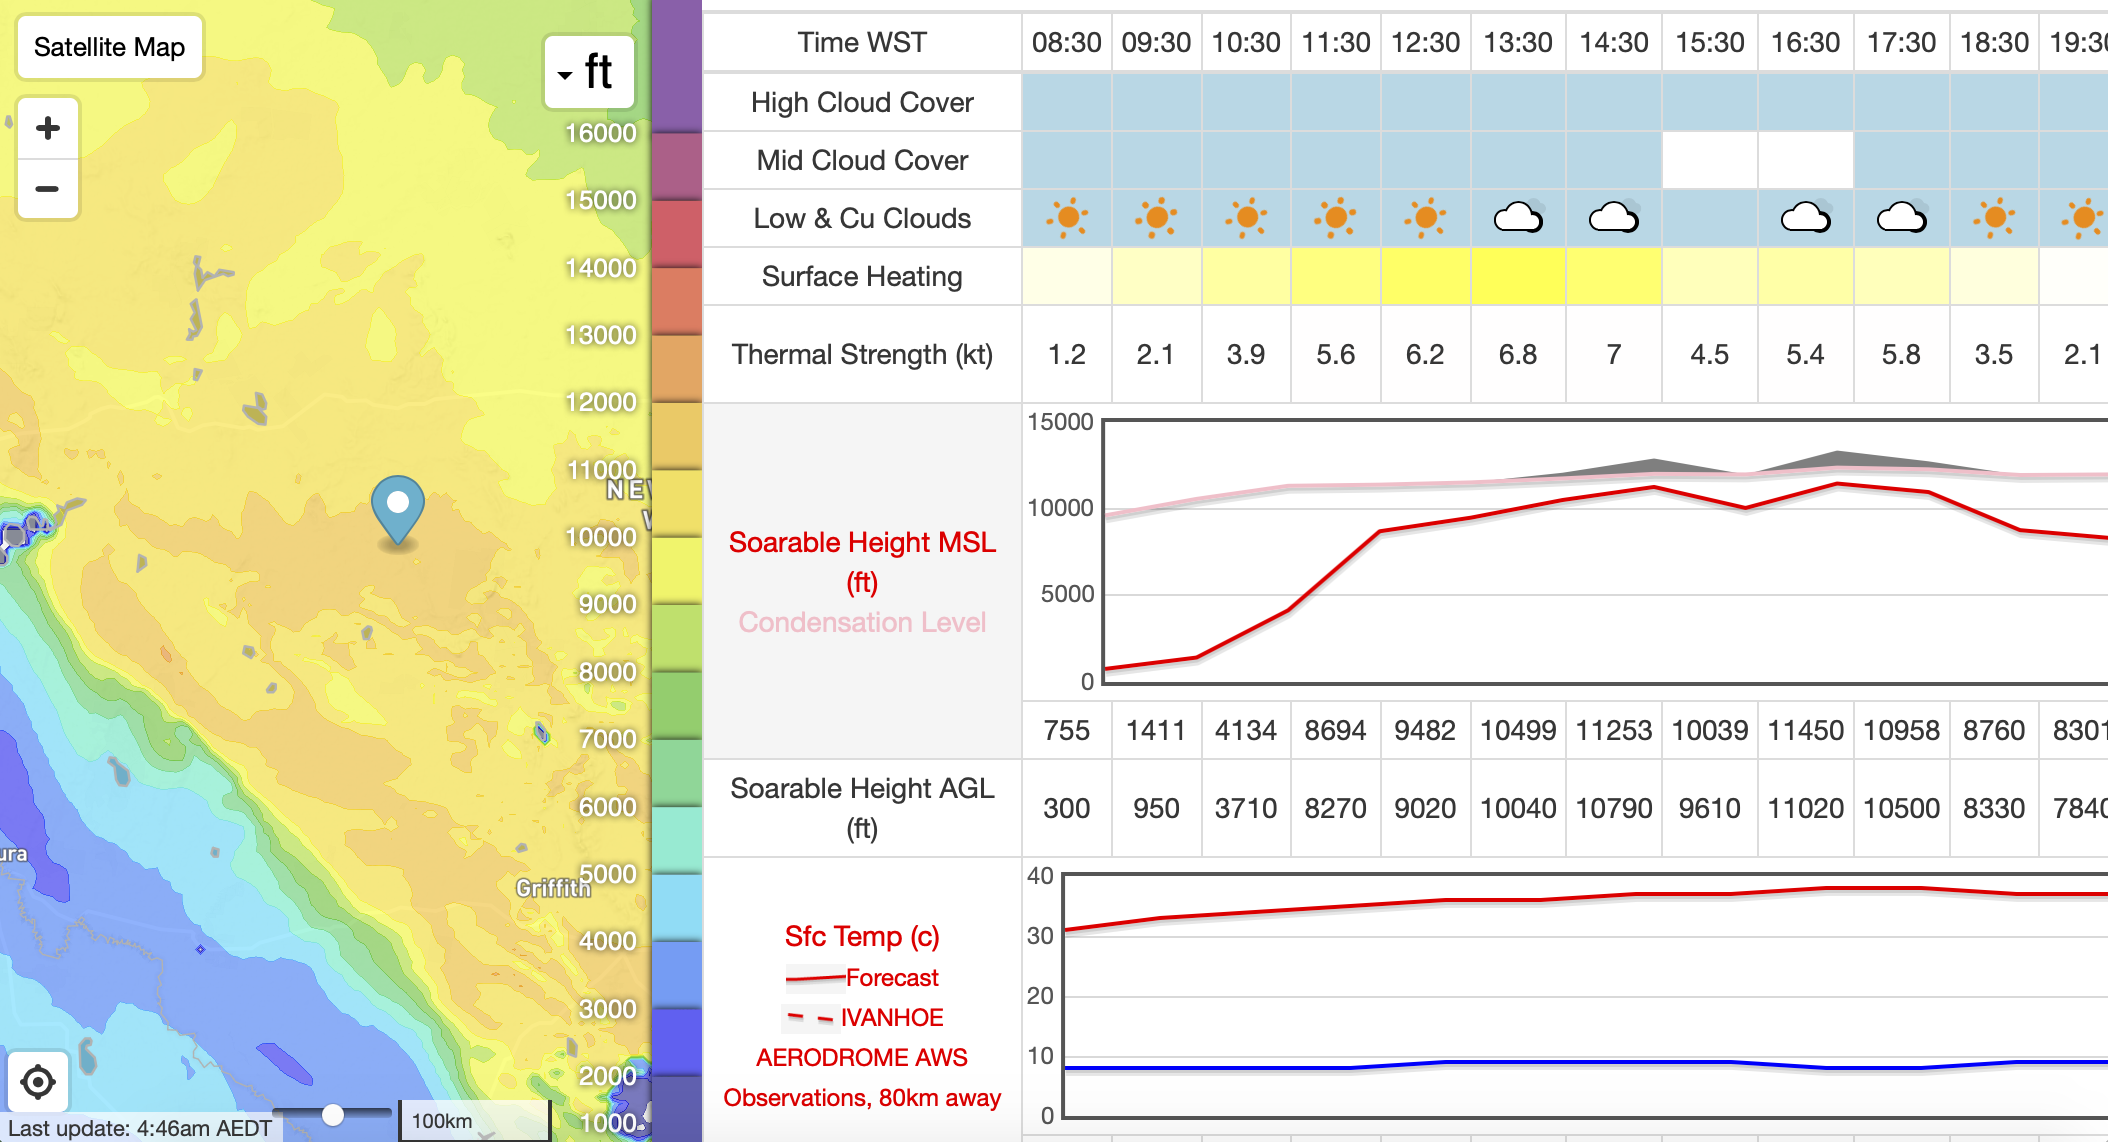
\includegraphics[width=\linewidth]{images/point_forecast.png}

The cloud cover is shown in the top rows with a colour gradient. Blue represents no cloud, whites are thin cloud, and darker greys indicate thick cloud.

Cumulus depth is represented on the convective graph with a dark grey shaded area above the condensation line. Where there is no dark grey shading, this suggests blue thermals.
\subsubsection*{
\includegraphics[height=15pt]{images/icons/windgram.png} Point Windgram}
The windgram shows the development in the lapse rate, temperature, relative humidity and wind throughout the day and with height at a point. This feature is useful to visualise inversion levels, moisture layers and wind shear.
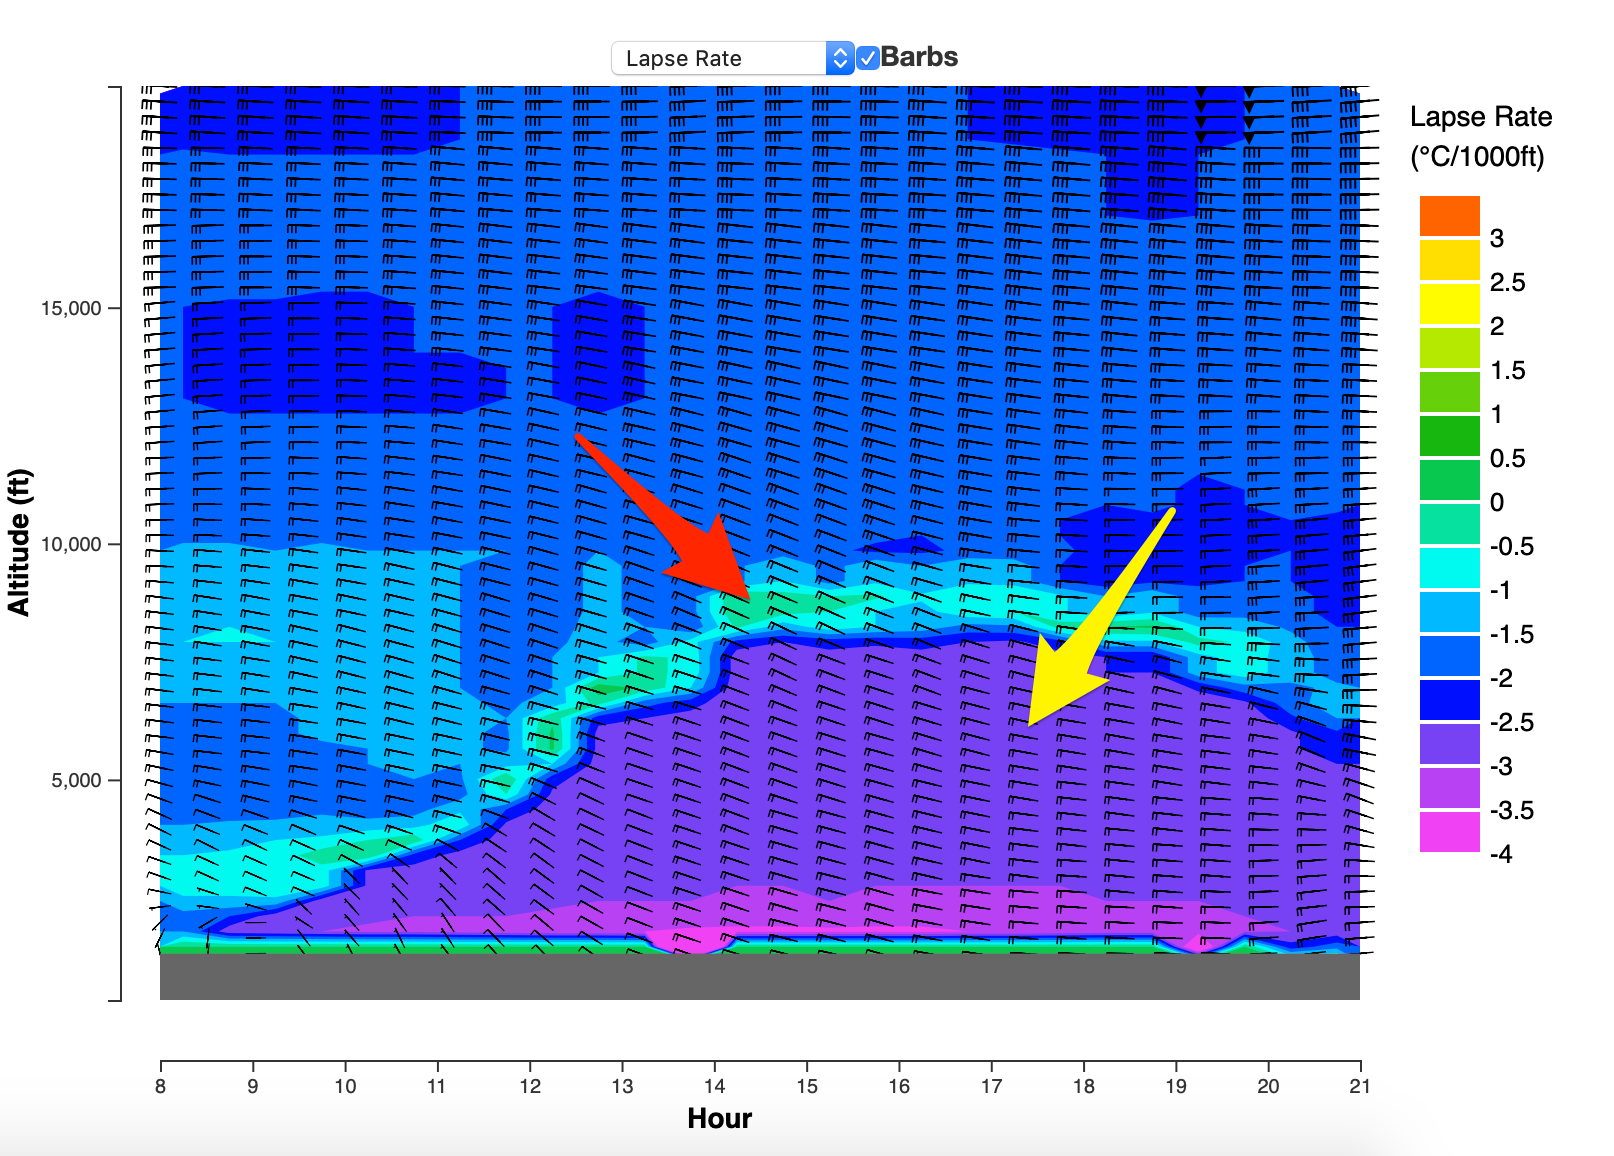
\includegraphics[width=\linewidth]{images/windgram_lapse_annot.png}
Using the Lapse Rate option, this shows a typical soaring day. As the inversion (
\includegraphics[height=11pt]{images/icons/arrow_red.png}) rises throughout the day, the convective layer (
\includegraphics[height=11pt]{images/icons/arrow_yellow.png}) becomes deeper.
\subsubsection*{
\includegraphics[height=15pt]{images/icons/route.png} Route Forecast}
The route forecast tool is able to estimate cross country speeds and summarise the forecast conditions over a planned task. The table on the right shows an estimated task speed for various times of day. Values of Inf. suggest the task may not be possible. This is a very useful tool to use during task planning and for competitions. By moving the points, it is easy to find the fastest and most realistic tasks for the day, and optimise the start time. You may have to move the points around to avoid unsoarable patches in complex weather in order to get a realistic task speed and solution.

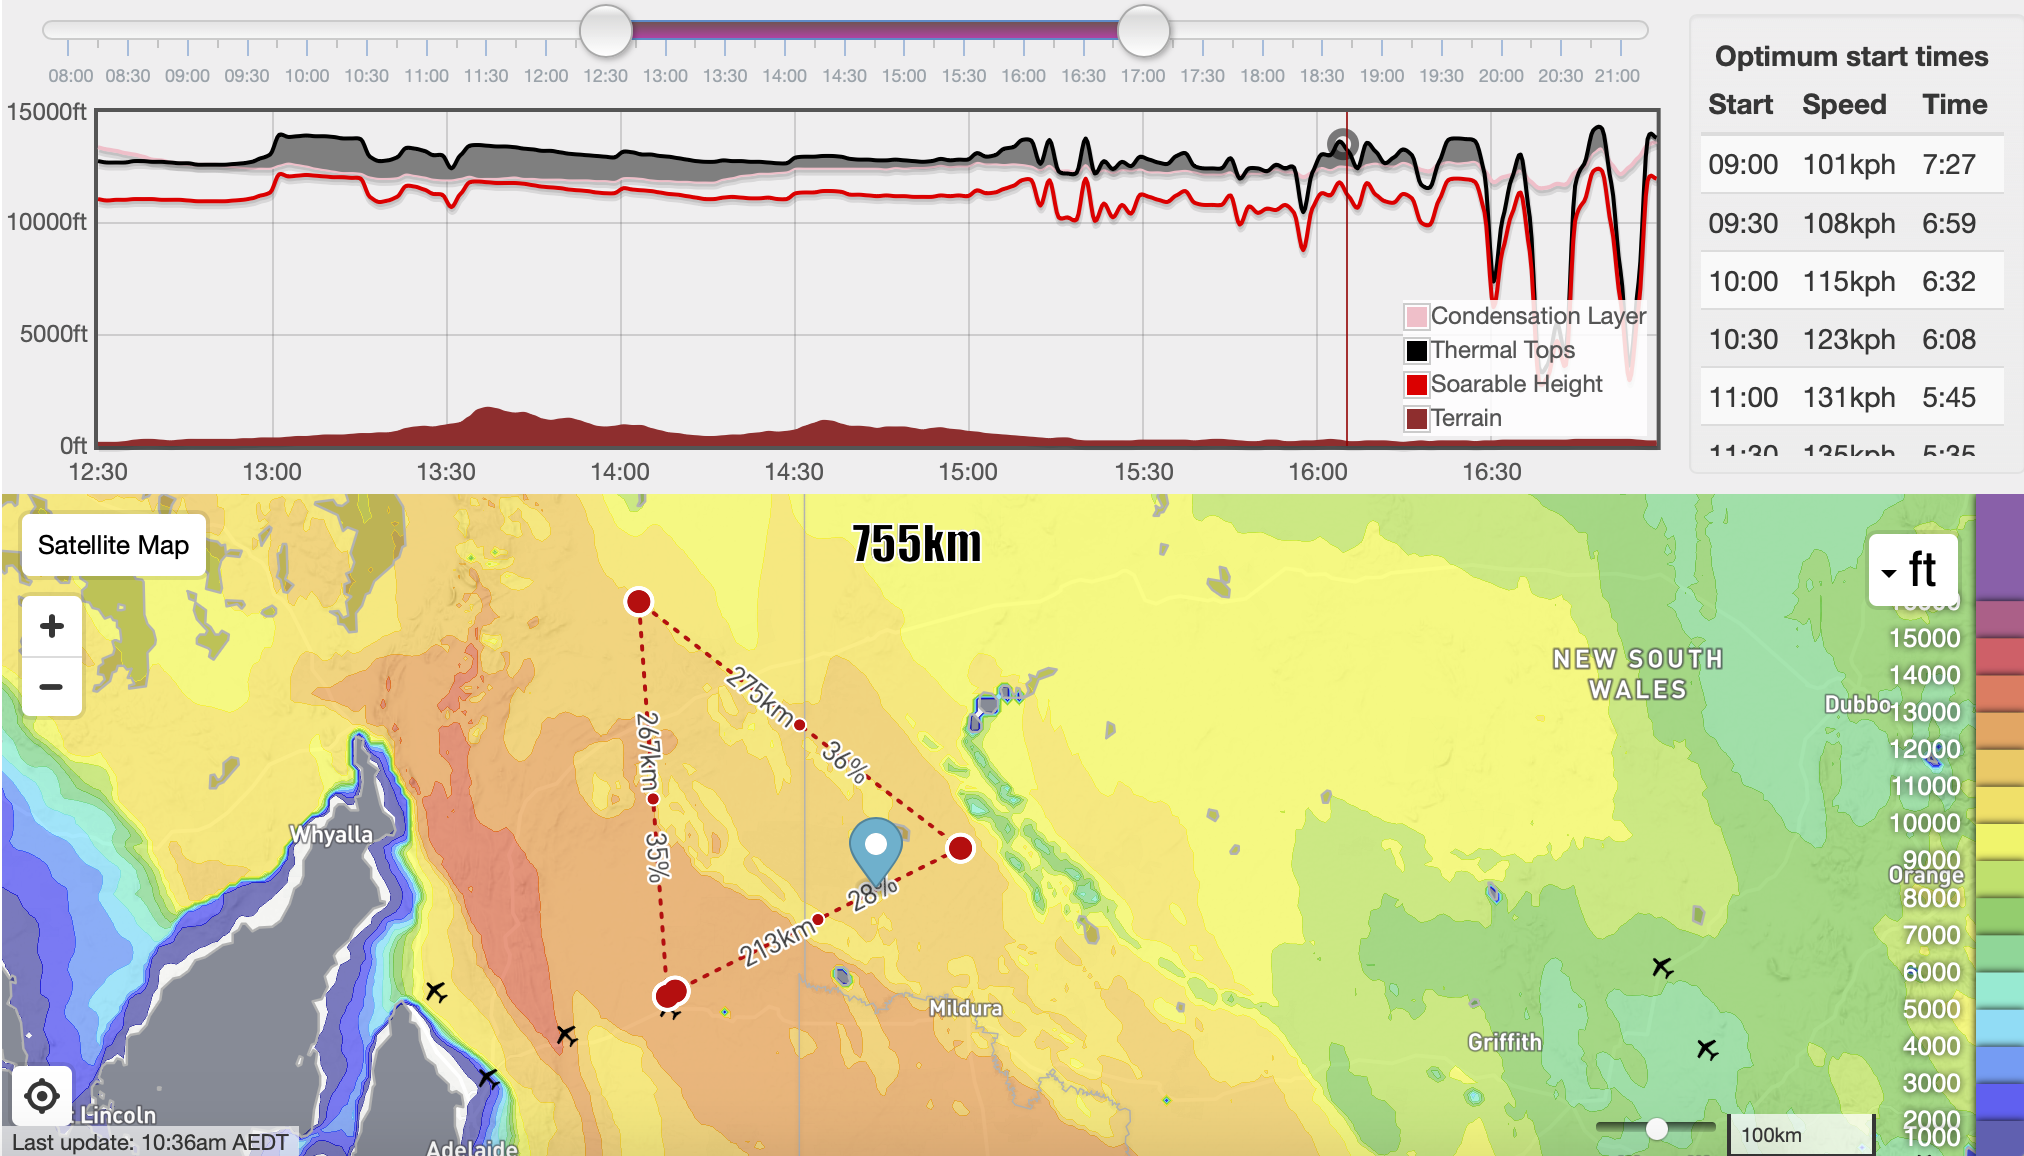
\includegraphics[width=\linewidth]{images/route.png}
\subsubsection*{
\includegraphics[height=15pt]{images/icons/wave.png} Wave Cross-Section}
The wave cross-section tool allows wave characteristics over height to be visualised. It gives a 2-D slice of the wave forecast between two points, with altitude on the vertical axis, distance along a line between the two points on the horizontal axis, and colours indicating vertical velocity. By drawing a line on the map perpendicular to the wave systems you identify with the Vertical Velocity plots from the parameter list.

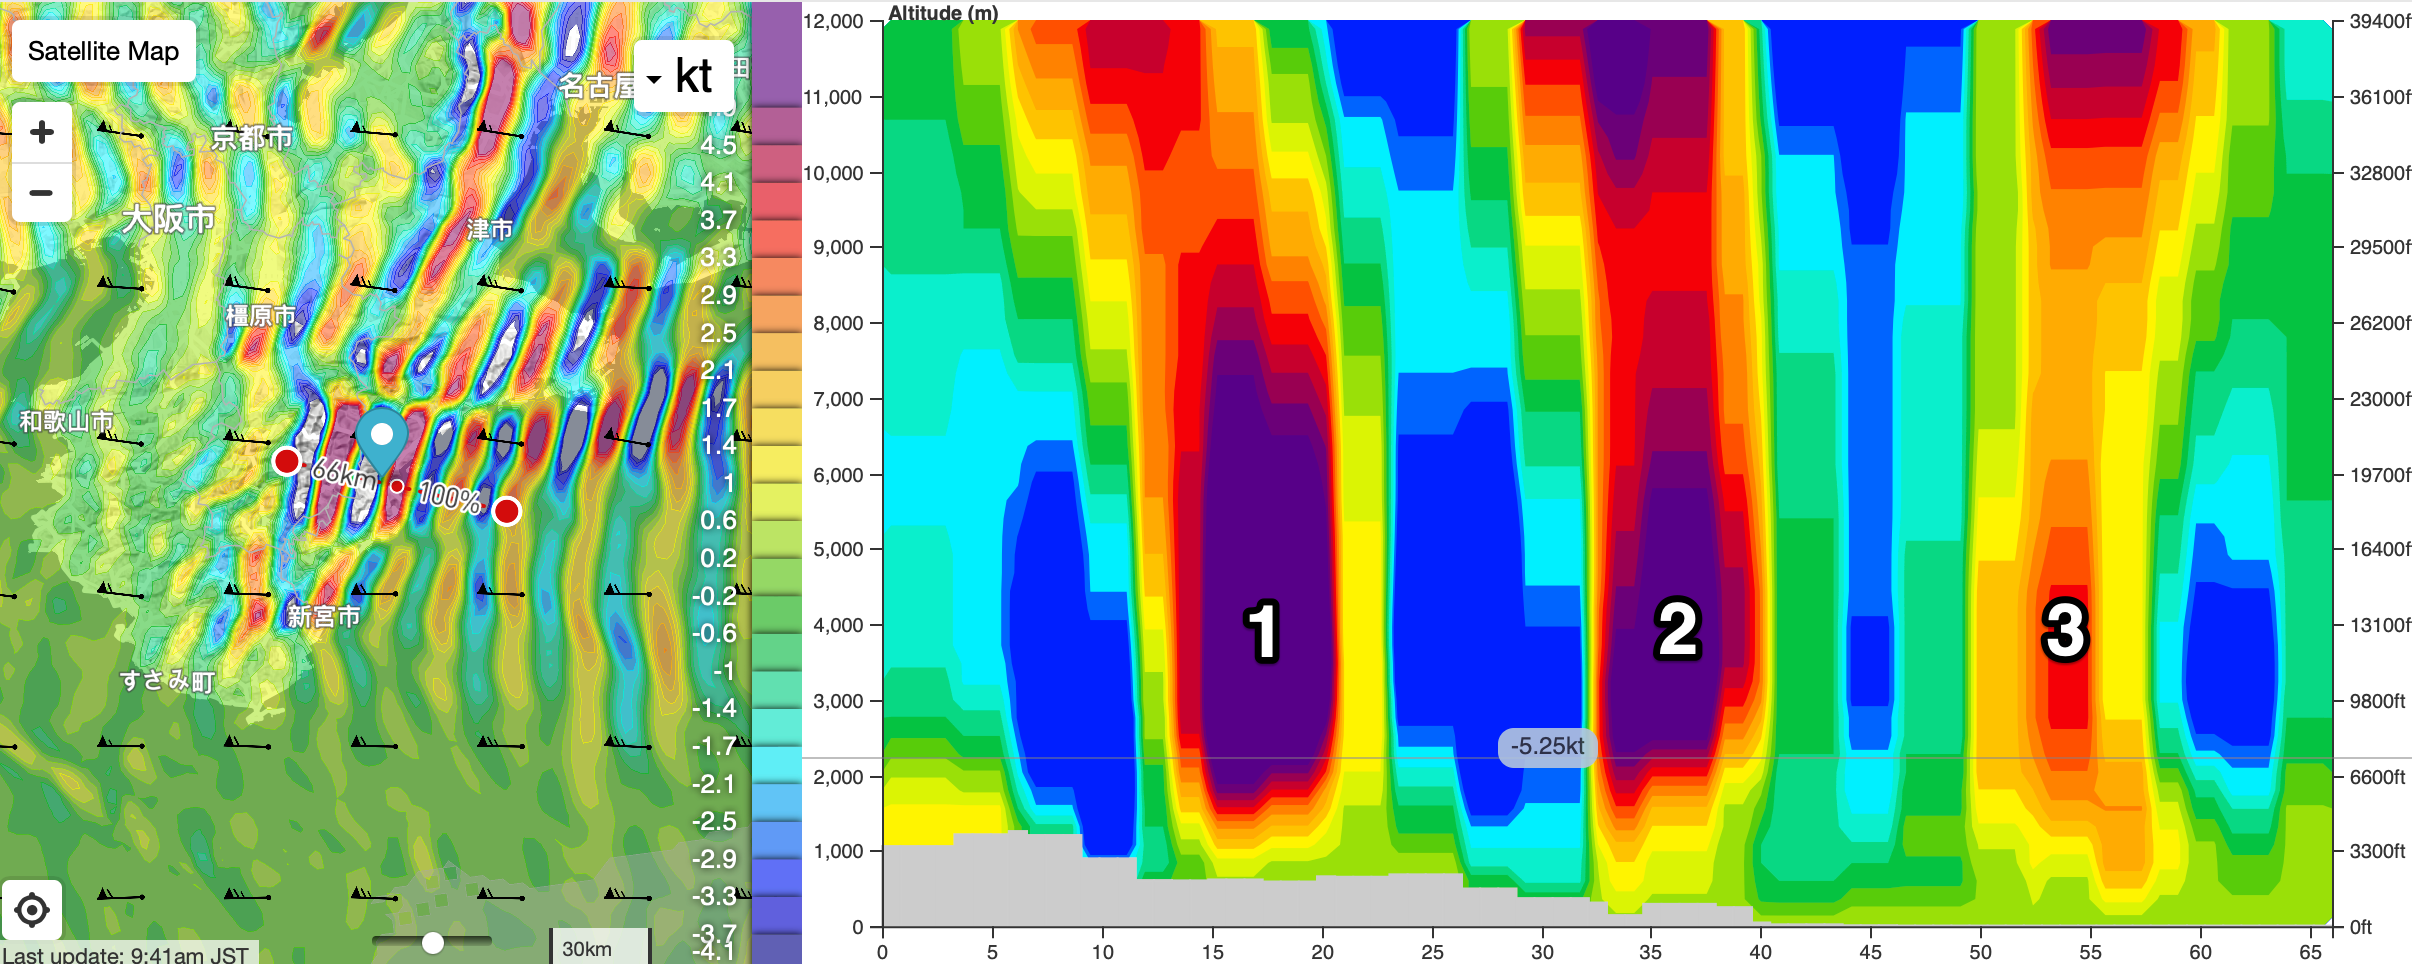
\includegraphics[width=\linewidth]{images/wave_x-section.png}

The chart above shows a Wave Cross-Section from the Japanese Alps. Region 1, 2 and 3 show the first, second and third waves, with reds and purples showing lift, and blues showing sink.

\subsubsection*{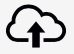
\includegraphics[height=15pt]{images/icons/igc.png} IGC Upload}
SkySight can be used as a post-flight analysis tool. This is a especially useful to confirm in-flight weather observations, and to help understand development and the interpretation of these in the SkySight forecast.

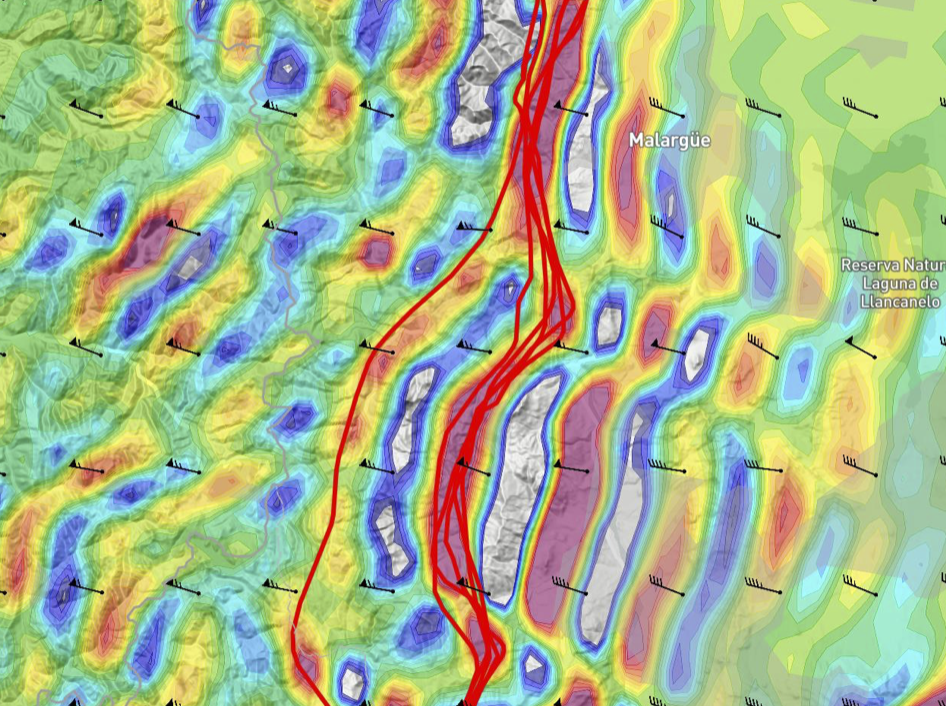
\includegraphics[width=\linewidth]{images/igc_upload.png}

\subsection*{How to access SkySight}
SkySight is available on both desktop and mobile platforms. It is accessible for a one week free trial and subscription at:\\
\url{http://skysight.io}



\end{document}
